\newcommand{\psd}[1]{{\small\sffamily{\color{blue!60}#1}}}

We reintroduce the problem from tutorial 1, an example of a 2D bar which
bends under its own load -- typical case of linear elasticity. The bar
\(5\times1\) m\(^2\) in area is made up of material with
\(\rho=8\times 10^3\), \(E=200\times 10^9\), and \(\nu=0.3\).

\begin{figure}[h!]
\centering
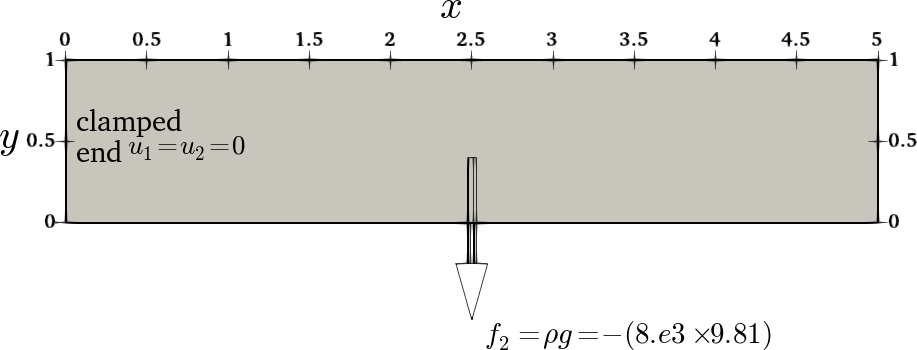
\includegraphics[width=0.5\textwidth]{./Images/le-2d-bar.png}
\caption{The 2D clamped bar problem. \label{2dbar-le-full}}
\end{figure}

\subsection{Step 1: Preprocessing}

First step in a PSD simulation is PSD preprocessing, at this step you
tell PSD what kind of physics, boundary conditions, approximations,
mesh, etc are you expecting to solve. More importantly for this tutorial
we will signify to PSD that MFront has to be used.

In the terminal \psd{cd} to the folder
\psd{/home/PSD-tutorials/linear-elasticity}. Launch
\psd{PSD\_PreProcess} from the terminal, to do so run the following
command.

\begin{lstlisting}[style=BashInputStyle]
PSD_PreProcess -problem linear_elasticity -dimension 2 -bodyforceconditions 1 \
-dirichletconditions 1 -postprocess u -useMfront
\end{lstlisting}

After the \psd{PSD\_PreProcess} runs successfully you should see many
\psd{.edp} files in your current folder.

\textbf{What do the arguments mean ?}

\begin{itemize}
\item \psd{-problem linear\_elasticity} means that we are solving linear elasticity problem;
\item \psd{-dimension 2} means it is a 2D simulation;
\item \psd{-bodyforceconditions 1} with applied body force acting on the domain;
\item \psd{-dirichletconditions 1} says we have one Dirichlet border;
\item \psd{-postprocess u} means we would like to have ParaView post processing files.
\item \psd{-useMfront} activates MFront interface for PSD.
\end{itemize}

At this stage the input properties \(E,\nu\) can be mentioned in
\psd{ControlParameters.edp}, use \psd{E = 200.e9}, and \psd{nu = 0.3}.
In contrast to tutorial 1, notice that these values of \psd{E} and
\psd{nu} are fed to a vector \psd{PropertyValues = [E, nu];} verbosed by
\psd{PropertyNames   = "YoungModulus PoissonRatio";}. We also signify
that we will be solving linear elasticity via
\psd{MforntMaterialBehaviour   = "Elasticity";} and also
\psd{MaterialHypothesis = "GENERALISEDPLANESTRAIN";} which signifies the
hypothesis to be used for the Linear elasticity
\footnote{The \psd{MaterialHypothesis} accepts \psd{"GENERALISEDPLANESTRAIN"},  \psd{"PLANESTRAIN"}, \psd{"PLANESTRESS"},  and  \psd{"TRIDIMENSIONAL"} as arguments.}.
\psd{PropertyValues}, \psd{PropertyNames}, and \psd{MaterialHypothesis}
will eventually be provided to MFront in \psd{FemParameters.edp} file
via \psd{mfrontElasticityHandler(...)} function
\footnote{User is encouraged to have a look at \psd{FemParameters.edp} file.}.
The volumetric body force condition is mentioned in the same file via
variable \psd{Fbc0Fy -78480.0}, i.e (\(\rho*g=8.e3*(-9.81)=-78480.0\)).
One can also provide the mesh to be used in \psd{ControlParameters.edp},
via \psd{ThName = "../Meshes/2D/bar.msh"}
(\textit{note that mesh can also be provided in the next step}) .In
addition variable \psd{Fbc0On 1} has to be provided in order to indicate
the volume (region) for which the body force is acting, here \psd{1} is
the integer volume tag of the mesh. Dirichlet boundary conditions are
also provided in \psd{ControlParameters.edp}. To provide the clamped
boundary condition the variables \psd{Dbc0On 2}, \psd{Dbc0Ux 0.}, and
\psd{Dbc0Uy 0.} are used, which means for Dirichlet border \psd{2}
(\psd{Dbc0On 2}) where \psd{2} is the clamped border label of the mesh
Dirichlet constrain is applied and \psd{Dbc0Ux 0.}, \psd{Dbc0Uy 0} i.e.,
the clamped end condition (\(u_x=u_y=0\)).

\subsection{Step 2: Solving}

As PSD is a parallel solver, let us use 4 cores to solve the 2D bar
case. To do so enter the following command:

\begin{lstlisting}[style=BashInputStyle]
PSD_Solve -np 4 Main.edp -mesh ./../Meshes/2D/bar.msh -v 0
\end{lstlisting}

Here \psd{-np 4} denote the argument used to enter the number of
parallel processes (MPI processes) used while solving.
\psd{-mesh ./../Meshes/2D/bar.msh} is used to provide the mesh file to
the solver. \psd{-v 0} denotes the verbosity level on screen.
\psd{PSD\_Solve} is a wrapper around \psd{FreeFem++} or
\psd{FreeFem++-mpi}. Note that if your problem is large use more cores.
PSD has been tested upto 13,000 parallel processes and problem sizes
with billions of unknowns, surely you will now need that many for the 2D
bar problem.

\subsection{Step 3: Postprocessing}

PSD allows postprocessing of results in ParaView. After the step 2
mentioned above finishes. Launch ParaView and have a look at the
\psd{.pvd} file in the \psd{VTUs...} folder. Using ParaView for
postprocessing the results that are provided in the \psd{VTUs...}
folder, results such as those shown in
figure\textasciitilde{}\ref{bar-le-full} can be extracted.

\begin{figure}[h!]
\centering
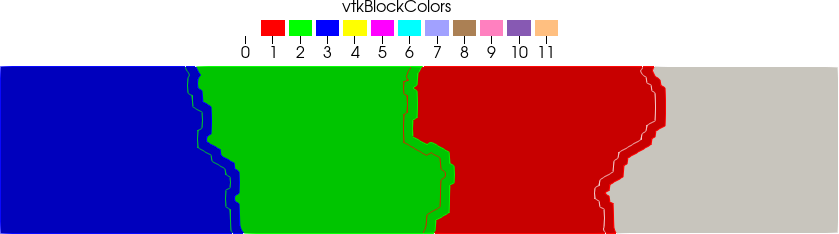
\includegraphics[align=t,width=0.4\textwidth]{./Images/le-2d-bar-partioned.png}\hfill
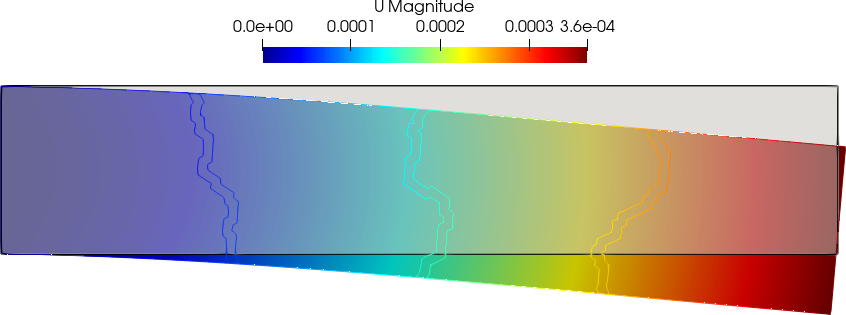
\includegraphics[align=t,width=0.4\textwidth]{./Images/le-2d-bar-results.png}
\caption{The 2D clamped bar problem: partitioned mesh and displacement field visualization in ParaView. \label{bar-le-full}}
\end{figure}

You are all done with your 2D linear-elasticty simulation with Mfront
interface.

\subsection{How and what is being done in PSD-MFront interface? }

To explain how PSD-MFront interface works we will compare how a PSD
solver acts when using MFront or without. In other words what is
different when \psd{-useMfront} is used at preprocessing. Note that
ultimately the problem results (displacement fields, stresses, strains)
will be the same.

To put it briefly, what MFront does for linear elasticity problem here
is build the Material tensor (stiffness matrix) at each quadrature
point. So, there are two points

\begin{itemize}
\item We need to communicate to Mfront the nature of the problem and the material involved.
\item We need to provide Mfornt the stiffness matrix at each quadrature point so that it can fill it up.
\end{itemize}

The two raised points are handled using
\psd{mfrontElasticityHandler(...)} in \psd{FemParameters.edp} file.

Firstly, the arguments \psd{E = 200.e9}, \psd{nu = 0.3},
\psd{MforntMaterialBehaviour   = "Elasticity";},
\psd{PropertyValues = [E, nu];},
\psd{PropertyNames   = "YoungModulus PoissonRatio";},
\psd{PropertyValues = [E, nu];} and
\psd{MaterialHypothesis = "GENERALISEDPLANESTRAIN";} form
\psd{ControlParameters.edp} takes care of the first point (the nature of
the problem and the material involved). The latter three arguments well
define that we have a 2D problem, with given values of properties
(\(E, \nu\)). The snippet from \psd{ControlParameters.edp} (produced
after using \psd{-useMfront} argument for \psd{PSD\_PreProcess}) file
shows these variables which define the nature of the problem and
characteristics of material involved

\begin{lstlisting}[style=CppStyle]
//============================================================================
//                   ------- Material parameters -------
// -------------------------------------------------------------------
//  E, nu : Modulus of Elasticity and Poisson ratio of the material
//  PropertyNames : String of material property names (space seperated)
//                  that are provided to Mfront.
//  PropertyValues : Values of material properties provided to Mfront
//
// -------------------------------------------------------------------
//  NOTE:     Please note that PropertyNames should be the same as
//            as in the Elasticity.mfront file
// -------------------------------------------------------------------
//============================================================================

  macro E()  200.e9  //
  macro nu() 0.3     //

  string    MaterialBehaviour  = "Elasticity";
  string    MaterialHypothesis = "GENERALISEDPLANESTRAIN";
  string    PropertyNames      = "YoungModulus PoissonRatio";
  real[int] PropertyValues     = [ E, nu ];
\end{lstlisting}

Secondly, the to get the stiffness matrix from Mfornt we use a
quadrature finite element space with vector finite elements built on it
(6 components) that represent the 6 components of symmetric material
tensor (\(\mathbb R^{3 \times 3}\)). The snippet from
\psd{MeshAndFeSpace.edp} file shows the 6 component Quadrature finite
element space for building material tensor.

\begin{lstlisting}[style=CppStyle]
//==============================================================================
// ------- The finite element space  -------
// ----------------------------------------------------------------------------
//  Qh       : Quadratur finite element space  for material tensor
//             FEQF2 implies 3 dof for a triangular cell in the mesh
//             A vectorial FEM space is built with 6 components
//==============================================================================

 fespace Qh  ( Th ,[ FEQF2, FEQF2, FEQF2,
                           FEQF2, FEQF2,
                                  FEQF2] );
\end{lstlisting}

Finally in file \psd{FemParameters.edp} the
\psd{mfrontElasticityHandler()} is called to build the material tensor
\psd{Mt} provided with the previously built material properties and
nature of problem. Please see the snippet below

\begin{lstlisting}[style=CppStyle]
//============================================================================
// ------- Material Tensor using Quadrature FE space -------
// -------------------------------------------------------------------
// Mt[int]  : is an array of finite element variable belonging to quadratu
//            re space Qh. This array is used  to define components of the
//            material tensor. 3X3 in 2D and 6X6 in 3D
//            In 2D the material tensor looks like
//
//         [ 2*mu+lambda ,  lambda      , 0 ]    [ Mt11 , Mt12 , Mt13 ]
//   Mt =  [ lambda      ,  2*mu+lambda , 0 ] =  [ Mt12 , Mt22 , Mt23 ]
//         [   0         ,     0        , mu]    [ Mt13 , Mt23 , Mt33 ]
//
// mfrontElasticityHandler : is a function in mfront interface that helps
//                           building the material tensor  Mt  given with
//                           material prpts.  from  ControlParameters.edp
//============================================================================

  Qh [ Mt11 ,  Mt12 , Mt13 ,
              Mt22 , Mt23 ,
                     Mt33 ];


  mfrontElasticityHandler( MforntMaterialBehaviour                             ,
                           mfrontBehaviourHypothesis = MaterialHypothesis      ,
                           mfrontPropertyNames       = PropertyNames           ,
                           mfrontPropertyValues      = PropertyValues          ,
                           mfrontMaterialTensor      = Mt11[]
                         );
\end{lstlisting}

Note that in the snippet above you might be seeing \psd{Mt11[]} being
provided as \psd{mfrontMaterialTensor}, in fact the \psd{Mt11[]} calls
the full matrial tensor not just the first component, so user should not
get confused
\footnote{This is more technical note, \psd{Mt11[]} is the cast of \psd{Mt} vector to a single array for memory optimization. One can also simply use \psd{Mt12[]}, \psd{Mt13[]}, \psd{Mt22[]}, ... all these are acceptable and are simply aliases to material tensor.}.

The material tensor \psd{Mt} built is used in the finite element
variational formulation to build the bilinear
\(a(\mathbf{u},\mathbf{v})\) which is used to assemble the finite
element matrix \(\mathbf{A}\) for the linear system
\(\mathbf{Ax} = \mathbf{b}\)

\[
a(\mathbf{u},\mathbf{v}) = \int_{\Omega}(
                 \varepsilon \left(\mathbf{u}):\mathbf{Mt}:\varepsilon(\mathbf{v}\right)
               )
\]

Here, \(\mathbf{u}:\mathbf{Mt}\) is nothing but the stress
\(\sigma(\mathbf{u})\) operator. User is encourage to have a look at the
\psd{VariationalFormulation.edp} file that contains the variational
formulation (weak form) of the problem described.
